\chapter{Solution Approach}
The system in this paper consists of three parts working together: The underlying financial structure, the third-party verification system, and Smart Sponsor for the actual donating process.
\section*{Verification}
If a user wants to prove they fulfill requirements they will need to show a form of proof. In this case, the verification uses a trusted third party. The verifier is represented by a smart contract on the blockchain that has an off-chain counterpart. Any user can request verification, be they an individual user or a business. \\
Before expanding on the verification process it is necessary to examine how conditions are structured. For the time being the conditions are represented as a singular string containing all conditions. This could be done in a form of JSON-format. This could also be represented by a smart contract. To prove that the user applying for a verification fulfills these conditions information will be exchanged outside the blockchain e.g. sending copies of certificates or pictures of identification. A person will then compare this information to the application and, if the information matches, submit a string into the smart contract of the verifier. The process to verify a condition is presented in Fig 3.1.\\
This submitted string is a hash over the conditions and the wallet address of the user. Every user can then look up the list of strings the verifier holds and see this one is contained. By using the hashed version, this string has no relevance to users who look it up, unless they have access to the conditions and the user address. Therefore, some of the privacy concerns of posting this verification on the blockchain should be alleviated.\\
\begin{figure}[H]
    \centering
    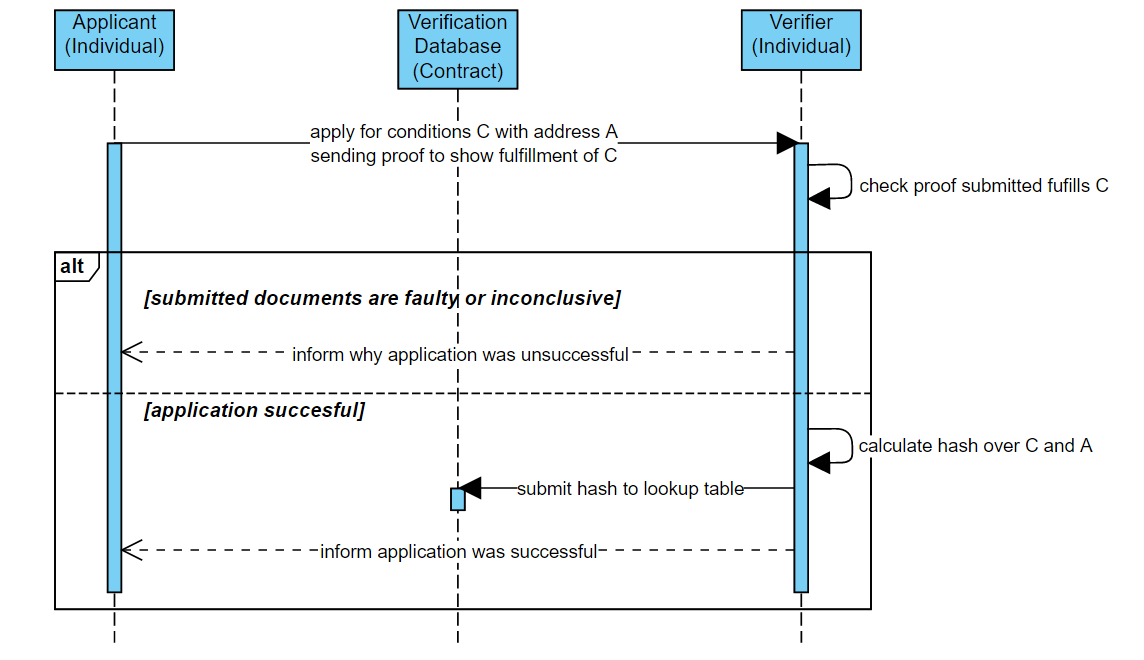
\includegraphics[scale=0.45]{figures/verification.PNG}  
    \caption{Verification process for any user}
    \label{fig:verifyModel}
\end{figure}
\emph{Remaining questions 1: When should the verification expire? How should the conditions be implemented? How will this lookup table be implemented?}
\section*{Underlying Financial Structure}
The underlying financial structure (from here on called the bank) uses tokens to represent fiat currency. It is represented by a smart contract on the blockchain. Fig 3.2. shows the structure of this smart contract and its relations to currency and users. As this is supposed to represent fiat currency a minting function is needed. At the same time there is an option to cash out tokens, burning these tokens \cite{pattern}. A token has two strings attached to it, one for sender conditions and one for receiver conditions. Ownership of these tokens is held in the smart contract of the bank including the transfer methods.\\
\begin{figure}[H]
    \centering
    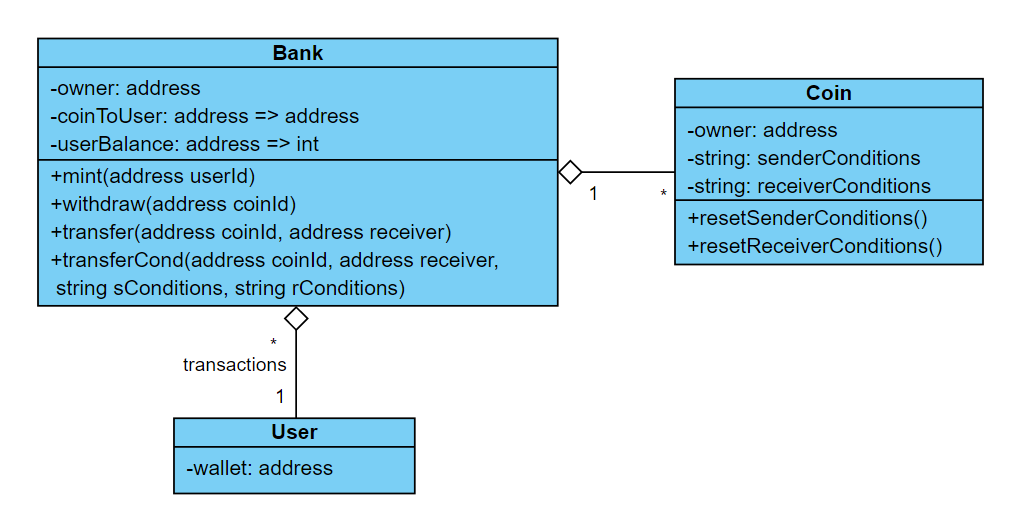
\includegraphics[scale=0.45]{figures/financeUML.PNG}  
    \caption{Class structure of the financial structure}
    \label{fig:financeUML}
\end{figure}
What differentiates these tokens from other systems, is the addition of a transfer method for adding conditions.
\begin{figure}[H]
    \centering
    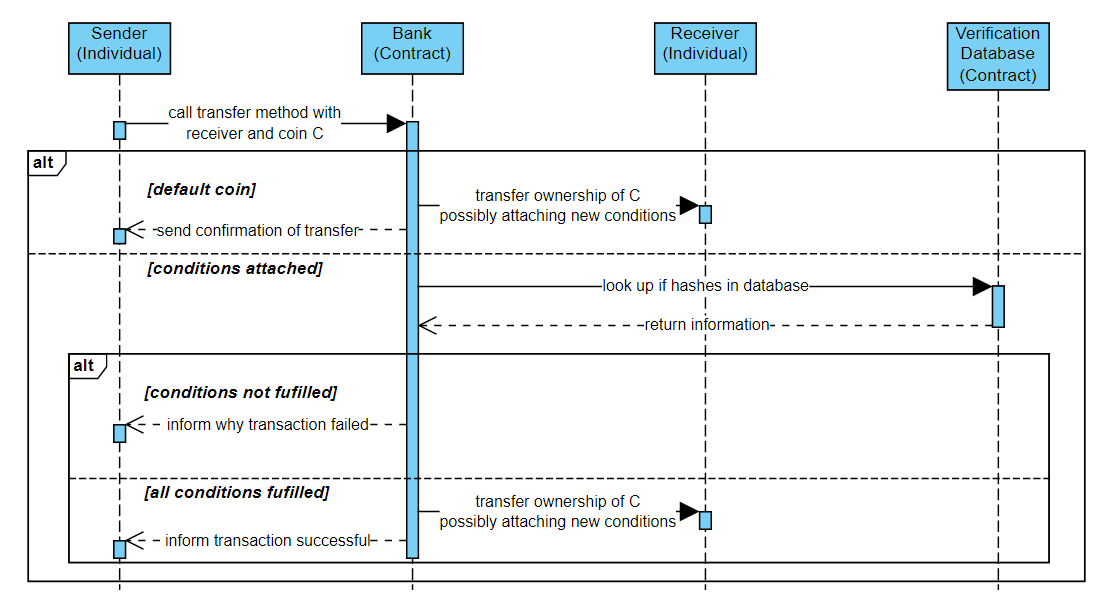
\includegraphics[scale=0.45]{figures/transfer.PNG}  
    \caption{Transaction process with possibility of attaching new conditions}
    \label{fig:transactionModel}
\end{figure}
This method, as detailed in Fig 3.3, transfers the token to the new owner and attaches conditions in the sender/receiver-condition attribute of the transferred coin.
As soon as conditions are attached to a coin, the transfer methods now need to reference if the resulting hashes are stored with the verifier.
If they are not, the transaction fails. It is possible to add further conditions to already existing conditions, but it should be impossible for a person who is not the one who sets conditions to remove them. Also, it should not be possible to turn tokens with conditions attached back into fiat currency.\\
\emph{Remaining questions 2: How long should conditions be attachable?}
\section*{Smart Sponsor}
Smart Sponsor is implemented as a smart contract. The donation process is depicted in Fig 3.4. The donor can set up a donation by transferring coins without attached conditions. The donor gives the conditions that should be applied separately and the smart contract saves these internally. Should a user apply for this donation, Smart Donor calculates the hash over the conditions and the wallet address of the applicant. It then checks if this hash is contained in the verifier's database. Assuming it is, Smart Sponsor then transfers the tokens while attaching the setup conditions.\\
\emph{Remaining questions 3: How can the donor be notified of how the money was spent? How can Smart Donor ensure the money is spent at all?}
\begin{figure}[H]
    \centering
    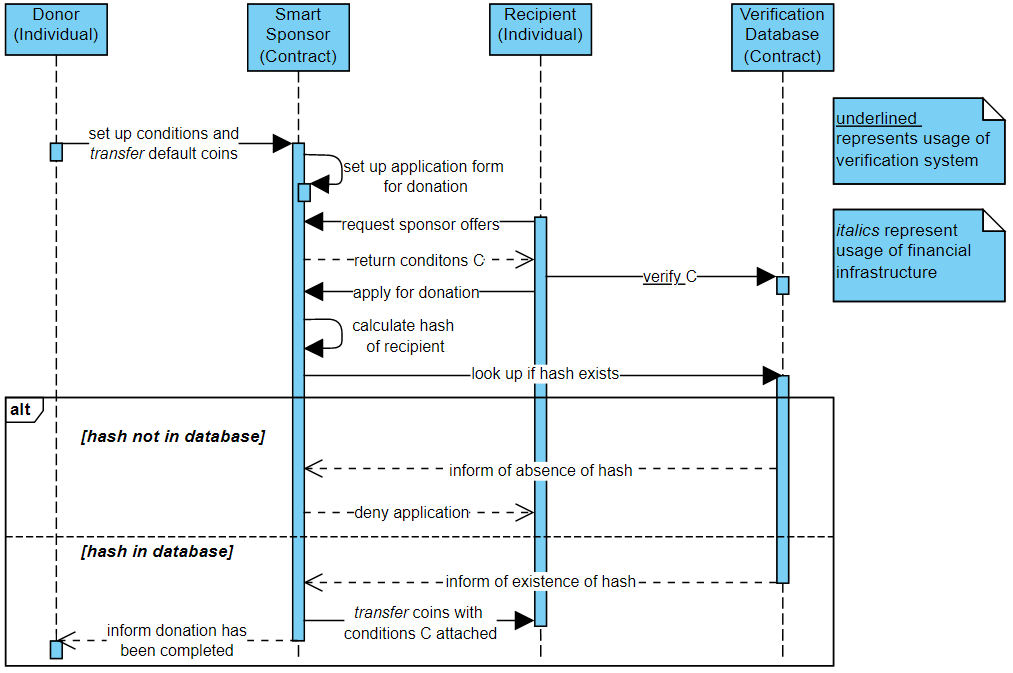
\includegraphics[scale=0.45]{figures/Smart Sponsor.png}  
    \caption{Process of donating currency with Smart Sponsor}
    \label{fig:donationModel}
\end{figure}
